\documentclass[pageno]{jpaper}

\newcommand{\IWreport}{2017}
\newcommand{\quotes}[1]{``#1''}


\widowpenalty=9999

\usepackage[normalem]{ulem}
\usepackage{graphicx}
\usepackage{adjustbox}
\graphicspath{ {figures/} }
\setlength{\parindent}{4ex}


\begin{document}

\title{
Drone Based 3-Dimensional Measurement and Analysis of Wireless Signal Propagation in Urban Environments}

\author{Pranav Badami\\Adviser: Kyle Jamieson}

\date{May 05, 2017}
\maketitle

\thispagestyle{empty}
\doublespacing

\begin{abstract}
Wireless mesh networks are an alternative means of home Internet delivery that could provide cheaper connectivity options for Americans. Connecting wireless links has its challenges due to obstacles and interference in the environment. This work proposes a robust, 3-dimensional measurement technique to assess the propagation of a wireless signal in an urban environment. The Drone Based Measurement (DBM) system collects spatial and spectral datasets and joins these into point clouds representing signal propagation. This system was used to measure wireless link propagation during a simulation in the Friend Center courtyard and, using aggregation-based analysis, found that the courtyard actually provides a more favorable configuration for signal propagation than an open field. The DBM system could be used to perform simulations around many other urban features, enabling new entrants into the wireless home Internet delivery space to build better mesh networks.
\end{abstract}
\pagebreak
\section*{Acknowledgments}
Professor Jamieson, thank you so much for your guidance and time throughout this process; I really appreciate it. 

Rishi, I don't even know how to express my gratitude. You helped me through the grind of this thesis and, without you, my morale would have been terrible. You're responsible for helping finish this thesis as much as I am.

Neil, thank you for sparking my intellectual curiosity about this topic; I'm extremely grateful for you doing so. Thanks for talking through parts of the project with me as we went along too. 

Purab, thank you so much for giving me your time to help with the crucial experimentation process. Sorry again about having you drive down just to get rained on. 

Mama and Didi, this was possible because of the support and freedom you guys give me. Thank you so, so much.

Lastly, thank you to the School of Engineering and Applied Sciences for their generous funding of this project. 
\pagebreak

\tableofcontents
\listoffigures

\pagebreak
\section{Introduction}
\subsection{The Problem: ISP Monopolies in the United States}
Home Internet users in the United States are at the mercy of their Internet Service Provider (ISP). Users seeking relatively modern download (> 25 Mbps) and upload (> 3 Mbps) speeds for home Internet are extremely restricted in their choices. The FCC states that 30\% of Americans (measured in developed census blocks) have no ISPs delivering home Internet at these speeds, while another 48\% of Americans have only one ISP providing service at these speeds\cite{fcc15}.

As a result of this lack of choice (and competition), American home Internet users are forced to pay disproportionately high prices for relatively slow connections. For example, Americans pay higher prices for home Internet than Europeans across all categories of broadband speed\cite{connectivity}(see Figure 1).

\begin{figure}[h]
	\caption[Comparison of broadband speeds, US vs Europe]{A comparison of prices for various categories of broadband speeds in the United States versus Europe.\cite{connectivity}}
	\centerline{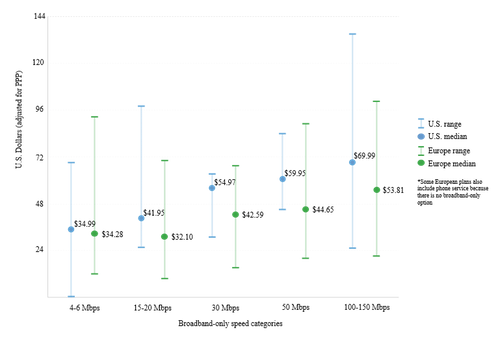
\includegraphics{comparison}}
\end{figure}

The plight of the American home Internet user is exposed even more when considering the highest available home Internet speeds for affordable Internet plans. While residents of Seoul and Hong Kong can choose among plans offering 300 Mbps connections in the price range of \$35-\$50 per month, no American city has any plans offering > 50 Mbps speeds for the same price range\cite{connectivity}. The much cheaper and faster connections available in Asia demonstrate that it is technologically feasible to provide fast home Internet connections for a low price. 

Not coincidentally, ISPs in Asia operate in a much more competitive landscape, forcing them to provide quality service at a lower price. In South Korea, for example, upstart ISPs can lease, and sell, unused bandwidth from a public utility that reaches the vast majority of the clustered, urban population. Further, the South Korean government forced Korea Telecom to open its network in the '90s, leading to increased competition and lower prices for users\cite{korea}. With so many options available to home Internet users, ISPs in Korea are forced to compete for customers on price and quality of service.

Unlike Korea, home Internet service in the United States is dominated by a handful of  major ISPs, which often collaborate to take advantage of the American Internet consumer. With fewer options available to them, the American customer is forced to except higher prices and low quality of service or go without home Internet altogether; this is not a viable alternative for many Americans.

The reason American home Internet delivery is dominated by a small oligopoly of ISPs is because of the prohibitive cost to set up fiber cable infrastructure. In contrast to Korea, the population of the United States is spread out over a vast expanse of land and reaching homes in the United States requires laying lots of costly wire, which is often expensive enough to deter all but the largest companies from attempting to provide Internet. Consider the efforts of Google Fiber. Google Fiber aims to offer connection speeds of 1000 Mbps at a comparable price to existing plans, reaching consumers in select neighborhoods of select American cities\cite{google}. According to Google, the process of bringing Fiber to a city involves initial exploration, network design, construction (laying fiber), and finally, customer sign up and installation. A Goldman Sachs report on Fiber, estimated that it would cost around \$140 billion for Google to cover the whole country\cite{goldman}. The involved process required to dig and install fiber is also extremely time consuming. The cost and time required to lay fiber across a wide geographic area makes it extremely difficult for even established companies like Google to enter the ISP realm, much less a host of smaller companies or startups. In 2014, Tom Wheeler, Chairman of the FCC, acknowledged the lack of competition among ISPs and recognized a need for the FCC to do more to protect and create competition in the United States\cite{wheeler}.

With a very small number of competitors entering the home Internet delivery space, the established ISPs are free to maintain the status quo and take advantage of Americans. If new, disruptively cheaper technologies could replace wired Internet infrastructure, businesses would be able to compete with the ISP oligopoly and provide better home Internet options for American consumers.

\subsection{A (Potential) Solution: Wireless Mesh Networks}
With the cost of establishing novel, last-mile wired networks being so high, there has been a lot of work on establishing cheaper wireless networks as an alternative delivery mechanism for home Internet. Wireless mesh networks are much more cost effective to set up because no digging is needed; nodes in the network are connected to each other by wireless links. With a low cost alternative technology, new businesses could enter the home Internet provider space and provide cheaper options for consumers. 

 One such notable project is Roofnet\cite{roofnet}, a wireless mesh featuring over 40 nodes spread out over the urban area of Cambridge, Massachusetts. Each Roofnet node consists of a small PC, an 802.11b card, and an 8 dBi omni-directional antenna. These nodes are primarily installed on three to four story tall buildings, with packets hopping wireless nodes until they reach a wireless node which is also connected to a gateway to the rest of the wired Internet. Individual users install these nodes on their roofs or windows and join the network. 

Similar to Roofnet, another community powered mesh exists in Red Hook, Brooklyn\cite{redhook}. The goal of these networks is to provide a cheaper, more accessible form of Internet architecture in comparison to the extremely expensive deployment of fiber cables. However, these wireless networks face challenges operating in the urban environment.

\subsection{Challenges with Wireless: Propagation and Measurement}
The propagation of wireless signals in a noisy, obstacle-ridden urban environment often results in wireless networks operating below peak efficiency. Buildings and other environmental obstacles, such as trees, can greatly increase the path loss of a wireless link between two nodes. Because of this, establishing a line-of-sight (LOS) connection between two wireless links is important for low-loss links and robust wireless networks. In addition, the Fresnel Zone (an ellipsoid-shaped volume) around the LOS must also be clear of obstacles for optimally low path loss between a transmitter and receiver. 

Measurement campaigns attempting to determine the impact of various environmental factors have taken very static approaches to gathering data in the past. Theodore S. Rapaport has conducted many such campaigns in a variety of settings in order to explore real-world propagation in different environments. For example, Rapaport, Durgin, and Xu's "Measurements and Models for Radio Path Loss and Penetration Loss In and Around Homes and Trees at 5.8GHz" was one such a campaign conducted in a suburban area. Signal strength measurement were taken by moving a receiver around a 1m square area and averaged to represent the path loss for a given room or outdoor location\cite{rapaport}. Such campaigns, while useful for sampling signal strength at key locations, don't give a complete understanding of signal strength over a larger space. 

Other campaigns have attempted to get a more complete measurement in an urban environment, but have been limited to measuring 2-Dimensions. A group of Brazilian researchers conducted a measurement campaign in Rio De Janeiro with a fixed transmitter on the window of an 8 story building\cite{urban}. They built a receiver block with GPS and collected measurements by driving around streets surrounding the building housing the transmitter. GPS and signal strength measurements collected by the receiver block were joined to construct a map of measured signal strength at street level, shown in Figure 2a . While this may be useful for mobile Internet users at the street level, participants in a wireless mesh for home Internet may have receiver nodes at various heights, necessitating a more 3-Dimensional measurement of signal propagation in urban areas. Manual campaigns, such as these, use labor intensive techniques commonly referred to as "war walking" or "war driving"\cite{urban}; these campaigns also have to be limited in scope due to the physical limitations of where measurements can be performed manually. 

One way to get a sense for propagation in 3-D is to use drone technology, an approach taken by several campaigns in the past. Drones offer several unique features that can make a measurement campaign more robust and complete than traditional static or manually measured campaigns because they can fly and be operated autonomously. Drones can be incorporated with measurement campaigns in a variety of different ways. For example, DroneSense\cite{dronesense} was an automated 3-D wireless signal measurement campaign created by a team of researchers from Dartmouth. The DroneSense system autonomously traversed indoor spaces using visual reference markers which trace a path through a space. These reference markers, shown in Figure 2b, are physically placed in a space and the drone uses its on-board camera and computer vision techniques to identify markers and use these markers to autonomously navigate through hallways and rooms. The drone's onboard wireless radio is used to measure signal strength.

\begin{figure}[h]
	\caption[Related measurement campaigns]{a (left): Continuous 2-D map of signal strength measurements in the streets of Rio de Janeiro\cite{urban}. b (right): DroneSense system navigating indoor space using reference points\cite{dronesense}.}
	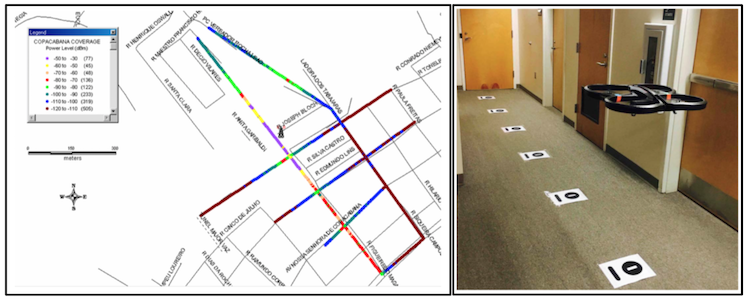
\includegraphics{related_work}
	\centering
\end{figure}

DroneSense has several issues that limit the scope of data it can collect. The DroneSense system can only measure signal strength in one frequency band because it relies on the drone's onboard wireless chipset; this doesn't allow the system to measure propagation under varying transmitter configurations. Regarding it's navigation module, DroneSense is limited in that it's navigation is reliant on physical reference points strategically arranged in 3-D space. This measurement technique is restricting in multiple ways. First, physical markers have to be created and laid out in 3-D space. While DroneSense is autonomous in terms of the drone's navigation, laying out the actual markers for the drone to navigate is still manual and limited by where markers can be placed. DroneSense also analyzes signal strength in terms of which reference point measurements were performed at. The reference points are points in 3-D space but do not have inherent spatial information encoded in them. So in addition to the manual placement of the reference points, DroneSense requires manual mapping of the reference points to 3-D space in order to create a continuous map of signal propagation. Lastly, DroneSense is limited to indoor measurement, where the measurement environment is much more contained and well behaved. 

\subsection{This Project: A More Robust Measurement Approach}
Common measurement techniques such as "war walking" and "war driving" don't provide robust, complete data that allow us to understand real-world signal propagation in complex urban environments. Newer approaches using drone technology, while promising due to spatially versatile, autonomous measurement, have also been limited in a variety of ways. Then, the question still remains: \textit{how can we gather more robust data to better inform the design of wireless mesh networks}?

Primarily, the data should help us form a complete picture of how a wireless signal from a transmitter propagates through a given environment. A crucial element of this is to perform measurements of signal strength in the complete 3-dimensional space. This is important because in a wireless mesh network, users may place transmitters and receivers in many different spatial configurations; for example, end users may live or work on different floors of apartment buildings and place antennas at varying heights. While DroneSense attempted to perform measurements in 3-D, their usage of reference points meant that their measurements were limited by the spatial arrangement of these points and the path the drone took to get to each of these points. Instead, a robust data set that would allow us to better understand real-world propagation would be a 3-D map of propagation through an environment.

Mesh networks can also be developed in many different environments, so a versatile measurement approach is also needed. Dense urban environments with taller buildings may necessitate a propagation map with emphasis on the vertical space between buildings. More spread out suburban environments with shorter buildings may require require measurement over large swaths of land. A robust measurement technique should be easily configurable to perform measurements in a variety of different environmental configurations. This versatile method would  depart from the conventional methods of war walking and war driving; there are many environmental configurations where it would be extremely demanding or impossible for humans to be physically involved in the measurement process. For the measurement technique to operate without direct human input, it would likely have to navigate autonomously. Drones are growing increasingly technologically capable and accessible; this technology could be strategically used to perform truly 3-D measurements autonomously. 

Experimental methodology is a  multi-faceted implementation choice that can greatly impact how insightful a signal propagation map can be towards real-world network configuration. Antennas in a mesh network can be placed in many different physical locations and operate with a variety of configurations. For example, transmitters can operate in different frequency bands depending on their circumstances. In urban environments, a signal in the 2.4GHz ISM band can provide better penetration through obstacles than a signal in the 5 GHz band; however, certain crowded channels in the 2.4 GHz may cause undesirable interference and require transmission in a less crowded channel. Experiments should account for these varying configurations and the measurement technique should also allow for measurement across commonly used ISM frequency bands. 

Lastly, there needs to be a digestible way to analyze the 3-D maps of signal strength across various experiments to determine which configurations worked better than others. This will require a combination of data visualization and data analysis. Visualizing the 3-D map can provide an intuitive understanding of how certain environmental features affect signal propagation in various configurations. Smoothing and aggregating the measured values over area or volume can provide metrics which help us digest the data and inform actual mesh network design.

\subsection{Drone Based Measurement (DBM): 3-Dimensional Propagation Mapping and Analysis}

Motivated by the desire to build more performant wireless mesh networks  in cities and suburbs, the drone based measurement (DBM) system aimed to develop a robust measurement technique to measure signal propagation in urban environments. We demonstrated the ability to create a 3-dimensional map of signal propagation in an urban environment; further, the DBM system was used to perform measurement experiments in different environments with various configurations, showing the versatility and extensibility of this measurement technique. Lastly, an analysis framework was developed to show how the 3-dimensional maps of signal strength, in concert with various experimental setups, can actually guide real world mesh network design. 

To do this, we built a signal measurement apparatus and flew it with a drone to conduct a measurement campaign in a handful of locations on the Princeton campus. A measurement apparatus collecting and storing signal strength measurements across either the 2.4 GHz or 900 MHz ISM bands was  mounted on a drone. We flew the drone on autonomous missions, where the drone created accurate, high-resolution flight data logs; over the course of a flight, these flight logs documented the drone's latitude and longitude coordinates with < 1 meter precision, along with the drone's height above ground. We then joined the drone's flight log data with the measured signal strength data recorded on our measurement apparatus. This joined data set allowed us to create 3-dimensional point maps of signal strength at frequencies across the 2.4 GHz or 900 MHz bands. The collected data was then aggregated to get a comprehensive, robust 3-dimensional map of signal strengths around a certain urban feature, such as a courtyard or a street with buildings on both sides.

There were two overarching research goals of this project. The first was to successfully generate a 3-D point cloud, as shown in Figure 3, with associated signal strength measurements in an urban environment. This data set served as the foundation for the subsequent research goals of the project. Experiments were ran with various transmitter locations and configurations, including varying center frequencies and channel widths; a separate 3-D point cloud was generated for each experiment. These sets of experiments were performed at a handful of locations across campus. Then, another important research goal of the project was to be able to spatially aggregate these point cloud data sets into "sections", or spatial buckets, where each bucket was assigned a value equal to the average signal strength of point measurements in that bucket. This served multiple purposes, making the data more intuitively understood and easily visualized. Also, this allowed us to normalize the data per unit of volume; normalized values can help compare the effect of certain transmitter configurations and environmental features on propagation.

\begin{figure}[h]
	\caption[Main research goals: point cloud and aggregation]{A mockup of the main research goals of the DBM system. Left: A 3-D point cloud of signal strength measurements, given a fixed position transmitter. Right: After analysis and aggregation, spatial buckets of average signal strength values are formed; this normalized data can be compared across experiments with various configurations.}
	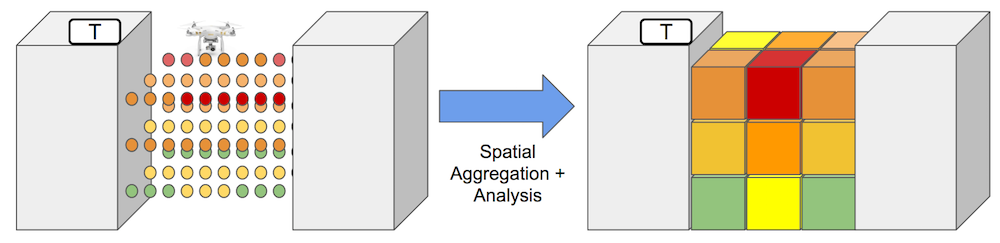
\includegraphics{measurement_goal}
	\centering
\end{figure}

This approach is novel because it yields a robust, 3-dimensional map of signal propagation; existing measurement techniques are restricted to 2-dimensional maps or static point measurements. Additionally, using a drone to fly autonomous missions and collect measurements made this approach viable in many different environments where war walking or war driving would be impossible. Since this project is motivated by wireless mesh networks,conducting measurements at various heights in challenging urban spaces is important as users can be situated at various floors. 
The analysis framework we proposed let us normalize and compare these complete 3-D data sets across many configurations to determine how best to layout a mesh network in an environment with certain features.

The remainder of this work discusses how the technological stack required by this approach was designed and built, and then proceeds to detail the methods of data collection and experimentation. Finally, it attempts to show how the proposed spatial aggregation analysis can inform better mesh network design in the future.

\section{Implementation: Point Cloud of Signal Strength Measurements}
Several implementation challenges presented themselves as we began to work towards the primary research goal. The following sections describe how we built the various components required to construct a 3-D point cloud of signal strength measurements. Mainly, transmitter configuration and receiver apparatus design are  important design choices for any measurement campaign.

\subsection{Transmitting a Wireless Signal}

\subsubsection{Transmitter Selection}
Since this project was focused on measuring the performance of wireless networks in urban environments, it was imperative to choose a transmitter which would be typically used in an urban setting. Consider a mesh network configuration in a town such as Princeton. This mesh network would need to meet several key criteria. First, it would need to have a way to connect to the wired Internet at some wired gateway, which could be many miles away or even in another town altogether. One reasonable way to establish this connection would be with the use of high-throughput, carrier-grade, long-range backhaul links which can establish wireless connections at ranges upwards of 100 km\cite{airfiber}.

End users of the mesh network living in Princeton would not be connecting directly to these backhaul links, however. Backhaul links would need to be placed at high elevations and meticulously aligned with one another to establish a LOS connection. It may be impossible for users to establish LOS connections with backhaul links because users will often have windows or roofs with obstructed views; further, they will also have pyhsically smaller, lower power antennas where they may not be able to transmit to a distant backhaul link.

Instead, a third kind of antenna is required to fill in the gaps between user bridge antennas and powerful backhaul links. A Point-to-Multi-Point (PtMP) link, which transmits to several receiving antennas, is required to complete the mesh network configuration. These PtMP links are more cost effective and smaller than backhaul links; they can be placed around the town of Princeton and serve as connection points for the end users who live on the same street, housing development, or intersection as one of these links.

For this project, the Ubiquiti NanoBridge M900\cite{nanobridge} will be used; the M900 is a PtMP link which operates in the 900 MHz spectrum\footnote{The decision to use a transmitter in the 900 MHz band is explained in Section 3.4 "Analyzing the PoC Propagation Data"}. The M900 is appropriate for an urban mesh network because it has good 180-degree coverage in the azimuth and elevation planes (see Figure 4). Then, if it is placed on top of a building facing the street, it can ideally provide a strong signal to a number of other buildings on the same street at a variety of elevations (floors); a large number of users would be able to connect to the M900 from their windows and join the wireless mesh.

\begin{figure}[h]
	\caption{Radiation patterns of the Ubiquiti NanoBridge M900\cite{nanobridge}}
	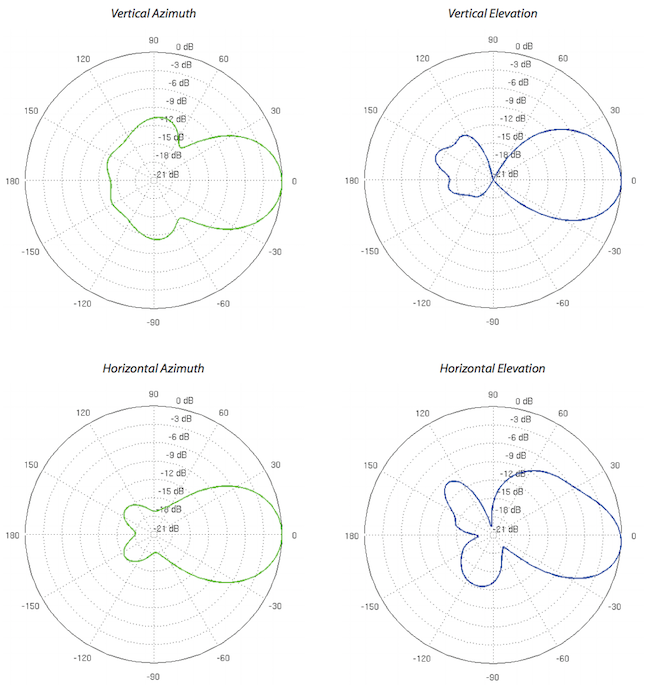
\includegraphics{m900_radiation}
	\centering
\end{figure}

Ubiquiti transmitters also allow for fast and easy configuration through the built-in airOS operating system. The airOS interface is accessed through a web browser and allows the user to change the operating mode of the device, the channel width, and the center frequency of the device; these parameters will be varied during the experimentation phase. For this implementation the Ubiquiti transmitter will receive power-over-ethernet (PoE) from a portable power supply and PoE adapter.

\subsection{Gathering Spatial Data with the Drone}
In order to create a 3-D point cloud of signal strength measurements, measured values need to be combined with 3-D spatial data. Two major implementation components are needed to achieve this goal. First, a drone is required to collect spatial data across various planes at many different heights. A signal measurement apparatus which can detect signals  across the 2.4GHz or 900 MHz spectrum and then record these measurements is also needed. If this apparatus can somehow be mounted on the drone, we could feasibly gather wireless signal data throughout a 3-D space. The data collected on these separate devices  can then be joined into a single data set representing the 3-D point cloud of signal strength measurements. 

\subsubsection{3-Dimensional Data: Collected via Drone}
Collecting precise and accurate spatial data would only be possible if a reliable  drone with state-of-the-art battery life could both log flight data and be autonomously controlled. Autonomous control is imperative to fly the drone in specific flight patterns, which can be overlayed on each other to produce the robust, complete dataset required for the 3-D point cloud. The DJI Phantom 3 Advanced\cite{p3a} is a "pro-sumer" drone which produces incredibly precise spatial data using multiple built-in stability and guidance systems. DJI is a world-leader\cite{dji} in producing drones for hobbyists as well as professionals. While other companies such as Parrot Drones\cite{parrot} sell devices with open-source hardware and software for increased customizability, this project used a DJI drone which was less customizable but more reliable. Reliability and fault-tolerance were key considerations because drone flights would be conducted in urban settings more prone to signal interference where drone failure could cause harm to property or people. Further, because of DJI's large market share, many third party apps leverage the extra features of the Phantom 3 Advanced that would potentially have to be created separately if another brand was used. 

Battery life was an important consideration because many autonomous flights would have to be conducted in a given space, each lasting several minutes. With an approximate 23 minutes of flight time out of the box, the P3A offers one of the longest flight times available in the consumer drone space. The P3A was used instead of the Phantom 4, a more recent model, because it has has a removable camera gimbal which was leveraged to build a mounting bracket housing the measurement apparatus (see Section 2.7, "Designing and Mounting the Apparatus"). 

\subsubsection{Spatial Data Collection}
The P3A features an optical stabilization system for micro-level positional adjustments and a robust satellite positioning system for macro-level navigation purposes. To measure height, DJI's "Vision Positioning System" (VPS) features two ultrasonic sensors and a monocular camera on the bottom-side of the drone.These sensors are always-on and the P3A uses the ultrasonic devices to measure distance from the ground and the camera to identify patterns under the drone; this input can be used to stabilize the drone such that it can hover in place or closely follow a pre-defined path. In addition, the P3A's satellite positioning system uses both GPS and GLONASS (the Russian satellite network) to provide geographic location services. The inclusion of GLONASS effectively doubles the number of satellites the P3A can fix onto; throughout testing and experimentation, the P3A was regularly fixed with 14+ satellites, providing robust, 1 meter accuracy. The geographic coordinates and the height measurements gathered by the satellite position system and VPS, respectively, are logged on automatically created flight logs and also transmitted to the drone's controller in real-time.

\subsubsection{Precision and Automation: Litchi iOS app}
Many third-party apps take advantage of these systems to provide autonomous navigation on the P3A. Litchi is an app which features a "Waypoint" mode where users can construct a path out of waypoints for the drone to follow (see Figure 5a). Custom heights and speeds can also be set for the waypoints; the drone's heading can also be manually controlled along the route. Specifically, Litchi allows the user to control the drone's heading using "points of interest"; for this project, the location of the transmitter will be a POI the drone will orient towards. At the start of a waypoint mission, the entire path is wirelessly uploaded to the drone which performs an auto-takeoff maneuver to begin the autonomous mission. The drone travels from it's starting location to the first waypoint and continues to follow the path until it reaches the last waypoint. 

\begin{figure}[h]
	\caption[Waypoints missions in the Litchi app]{a (left): Waypoint mode in the Litchi app, viewing a mission. Purple markers denote the waypoints, which the drone will traverse in numbered order. The clouds above each marker indicate the height the drone should assume at a given waypoint. The opaque blue paper airplanes under the waypoints indicate the drone's heading. The blue marker is a point of interest. b (right): Path followed by the drone during a test of this waypoint mission; the drone took from the H (home) marker. Note that waypoints are separated by < 16 ft, demonstrating the granular position control of Waypoint mode.}
	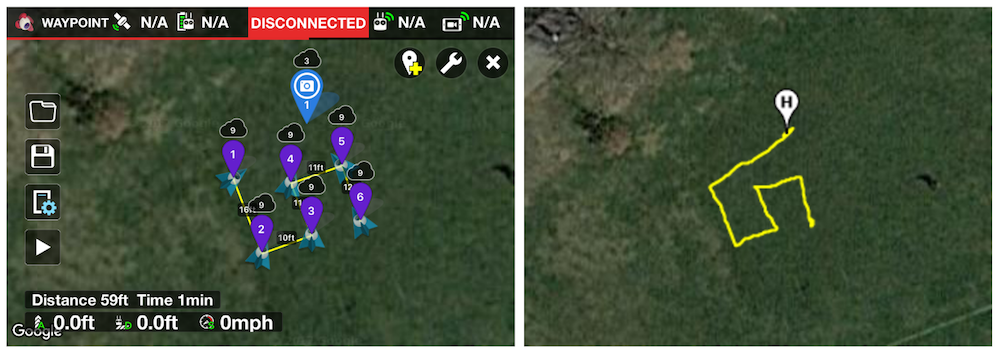
\includegraphics{waypoint}
	\centering
\end{figure}

The Litchi app also integrates with AirData UAV to automatically sync flight logs after each completed flight (see Figure 5b). AirData UAV serves as a repository that allows users to download flight logs much more easily than accessing the internally stored flight logs on the P3A. Data can be downloaded in CSV format for ease of analysis, or KML for ease of integration with mapping services such as Google Earth. Logs (Figure 6) include timestamped information collected from the drone's built-in systems, include the machine's height, latitude and longitude. Geographic data is reported in decimal notation, while timestamps are in UTC-3 format. Litchi flight logs also contain fields detailing how long the machine has been flying (in milliseconds) as well as the flight state; since missions occur autonomously, the drone takes-off and lands automatically and records these maneuvers as distinct flight states. When the drone is traversing between waypoints, it logs a dedicated waypoint fly state, allowing for a convenient way to filter data when constructing the point cloud. 

\begin{figure}[h]
	\caption[Example flight log from the Litchi app.]{An example flight log from the Litchi app, automatically synced to and downloaded from the AirData UAV repository. Note the change in the "flycState" column as the drone transitions from taking-off to executing a mission. (This is only a small subset of columns from the flight log.)}
	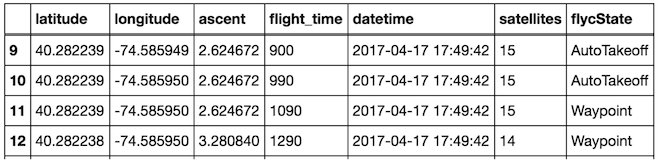
\includegraphics{flight_log}
	\centering
\end{figure}

\subsubsection{Drone Safety: Features and Precautions}
Since drone flights would be conducted on the Princeton campus, we had to be certain that the drone would take appropriate fail-safe measures in case something went wrong during an experiment. For example, the connection between the drone controller and the aircraft is a wireless connection in the 2.4 GHz band; what would happen if the connection between controller and aircraft was broken due to heavy interference? Or simply if the controller battery died?

First, we tested how the drone would perform if it lost connection to the flight controller during a manual flight. The drone's behavior in this scenario can be configured in the aircraft settings menu through both the DJI GO or Litchi apps. Since the drone would not be flying directly above buildings, obstacles, or people during our experiments, it was configured to perform and auto-land maneuver if connection with the controller was lost. To simulate losing connection with the controller, we simply turned the controller off while the drone was in flight. This was tested 3 times and the drone landed successfully each time. 

We also wanted to test how the drone would perform if it lost connection with the controller during an automated waypoint flight. This behavior can be set in the mission settings menu in the Litchi app. Since the drone auto-lands once it reaches the last waypoint of the mission, we opted to configure it to auto-complete the mission even if it lost connection with the controller. We tested this 3 times and the drone successfully completed it's mission each time. 

When the drone is performing automated flights in waypoint mode, the controller is set to Function, or "F", mode; manually controlled flights occur when the controller is in Positioning, or "P", mode. Another potentially unsafe scenario could be when the drone malfunctions (possibly due to a compass or VPS error) while the controller is in "F" mode and manual control is disabled. We wanted to ensure that switching the controller to "P" mode would successfully restore manual control of the aircraft in case it needed to be steered out of danger and landed. Switching modes and landing the craft was tested successfully three times as well.

\subsection{Receiver Apparatus Overview}
At a high level, the receiver apparatus would need to measure and log signal strength across the 2.4 GHz or 900 MHz bands. Furthermore, it would also need to log timestamps for these measurements; this is because the spatial data on the drone would need to be joined with the spectral data from the apparatus to generate the desired point cloud of signal strength. Aggregating and comparing this point cloud data could inform best practices for transmitter and/or receiver placement in various urban settings.

The receiver apparatus (see Figure 7) was built on a light wood board and contained a Raspberry Pi, spectrum analyzer, and a portable battery pack; a measurement and logging script ran on the Raspberry Pi to collect and store data. The design of the receiver apparatus was heavily constrained by weight; in total, the receiver apparatus weighed 246.9 g. If we were to mount the apparatus on a drone, it would certainly need to be light enough for the drone to fly and be controlled reliably. Another important constraint was the ability to interface with the equipment, since the collected data needed to be logged for later analysis. The following sections describe each of these design elements in more detail.

\begin{figure}[h]
	\caption{Layout of the receiver apparatus, which is to be mounted on a DJI Phantom 3 drone.}
	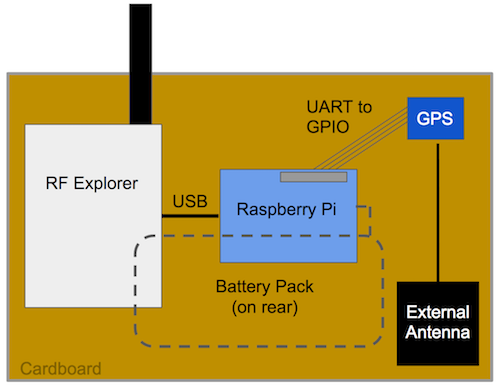
\includegraphics{apparatus}
	\centering
\end{figure}

\subsection{On-board Computing and Logging}
A Raspberry Pi 2 Model B served as the on-board computer of the receiver apparatus. The Raspberry Pi was selected for it's versatile interfacing options and expandable flash storage, as well as it's very light weight (44.5 g), power efficient design (200mA operating current). Specifically, the Model B\cite{rpi} has 4 built-in USB ports as well as 40 General Purpose Input/Output (GPIO) pins. The Pi ran a Raspbian Jessie operating system mounted on a 64 GB SD card, which stored the collected data. To power the Raspberry Pi, a lightweight (79 g) lipstick battery with a capacity of 3350 mAh was used; this meant that the Pi could be powered for many hours at a time, which was a crucial feature later required to perform experiments (see Section 3.1, "Setup and Flight Planning"). 

\subsection{Spectrum Analyzer}
The receiver apparatus needed to have a spectrum analyzer to measure the strength of wireless signals in the 2.4GHz or 900 MHz bands. This project used the RF Explorer handheld spectrum analyzer, a relatively lightweight device (185g with casing) that can run off its own internal battery and features a mini USB port for interfaceability\cite{rfe}. RF Explorer allows for easy configuration of minimum and maximum frequencies detected as well.

To collect data from the spectrum analyzer, the RF Explorer was connected to a Raspberry Pi(see "Logging and Compute") with a serial connection over USB. The RF Explorer sends bits over the serial connection; these bits are structured as "sweeps" of signal measurement data.  On each sweep, RF Explorer sends the measured signal strength for frequencies from its configured minimum to maximum frequency. 

RF-Explorer-For-Python (RFEP) is a Python library with an API for detecting, connecting to, and reading from an RF Explorer device. Upon instantiating a RFECommunicator object provided by RFEP, the user can connect to the RF Explorer by configuring the RFECommunicator connection as a serial connection with the appropriate USB device port. The RFECommunicator then provides utility functions to read sweeps of spectral data, returned as arrays of dBm values, where each index corresponds with a step frequency increase from the index before. This functionality will allow us to simultaneously gather and log signal strength data across the transmitting frequencies of our PtMP link, as determined by the transmitter's configured center frequency and channel width.

\subsection{Measurement and Logging Script}

In order to construct the 3-Dimensional map of signal propagation, the receiver apparatus would need to gather data from the spectrum analyzer and log this data in the Raspberry Pi's onboard filesystem. As mentioned earlier, the spectrum analyzer communicates with the Pi over a serial connection.

First, data from the RF Explorer was collected at 50000 baud via the USB serial connection using the RFECommunicator object from the RFEP library. The RFECommunicator object featured several convenient utility methods to get parsed signal strength data in an array. The measurement script initially connected to the RFE and configured it as necessary for any given experiment that had to be performed. After a serial connection over USB was established, the RFE measurement configuration was read, allowing us to fix the minimum frequency and the step frequency. The first value in an array of sweep data corresponded to the signal strength at the min frequency while the value at some index $i$ corresponded to frequency $min_freq + i*step_freq$. After setting these configuration variables,  the measurement script entered a \texttt{while} loop where it continuously read data from the spectrum analyzer as new sweeps of data became available.

Frequency and signal strength were logged as timestamped rows (using python's \texttt{datetime}) in a file in the Raspberry Pi's filesystem. To increase the utility of the data collected on the measurement apparatus, the Pi logged measured signal strength at every frequency step in every sweep gathered by the RFE. The RFE had an update rate of around 5 Hz; a test run counting the number of RFE sweeps in 100 seconds returned a tally of 519 sweeps, including the few seconds required for the RFE to set up and begin sampling its configured frequency band. Based on this update rate, the measurement script logged approximately 1 MB of data per minute of runtime. 

The timestamp of each logged row was as crucial as the spectral data contained in the row because measurement data would be joined with spatial data from the drone using timestamps. Initially, the apparatus included a GPS module connected to the Raspberry Pi with a serial GPIO connection; this enabled us to log spatial and spectral data collected simultaneously in the same row because all the data was flowing through a single script on the Pi. However, positional data collected using the Pi was extremely unreliable compared to the robust data logged on the P3A; using the drone as a source of data then necessitated having to join data collected on separate systems.

 One implementation challenge that presented itself was the lack of a real-time clock (RTC) on the Raspberry Pi, which necessitated manual clock alignment before measurement could begin. Due to the omission of an RTC, the Raspberry Pi defaulted to its factory time setting whenever it booted and kept time from that point using a quartz crystal. On the other hand, the P3A logged accurate time in the UTC-3 timezone. To align the Raspberry Pi, the Network Time Protocol, or \texttt{ntp}, synchronization service had to be invoked when the Raspberry Pi was connected to a network over Ethernet. Once synced and disconnected from the network, the Pi had to remain on so it would not reset to its factory default time. 

\subsection{Designing and Mounting the Apparatus}
The receiver apparatus had to be mounted to the P3A in order to take measurements at various heights in a 3-D space. Unfortunately, the P3A is not designed with payload capacity as primary consideration; it is rated as having a low carrying weight of 300g\cite{dji}, in addition to its internal components. The more weight the P3A is carrying, the shorter it's flight time and reliability is. Since the P3A, is sold as a photography device, it comes with a camera gimbal assembly already mounted under the drone. The first step was to detach the camera gimbal from the underside of the drone, revealing the mounting bracket attached to the body of the P3A.  See Figure 8a for the exposed mounting bracket. With the gimbal removed, the P3A could then be operated in the same way as before; the only difference in functionality was that no video was streamed from the aircraft to the controller. Manual and automated flight modes continued to funciton as described previously. 

 Once the gimbal was removed, several design choices regarding the design of the apparatus presented themselves. The measurement apparatus consisted of the three components: the Raspberry Pi, the RF Explorer spectrum analyzer and the Anker lipstick battery needed to power the Pi. One option was to secure these components to the body of the P3A separately; however, the Pi needed to be connected via USB cables to the other devices. Rather than have the devices taped individually around the aircraft, requiring loose wiring to connect them, we chose to create a lightweight mounting platform that would securely fix to the now vacant bracket formerly occupied by the camera gimba.  
 
\begin{figure}
	\caption[Preparing the drone and mounting the apparatus]{a (left): Preparing the P3A for mounting. First, the camera gimbal is remove to expose a mounting bracket. Note the protruding VPS unit at the rear of the craft, which needed to remain unobstructed for stability. b (right): Mounting the apparatus to the bracket. Note the constraints imposed by the spacing of the holes in the bracket. The P3A had a tested payload capacity of 300 g.}
	\centerline{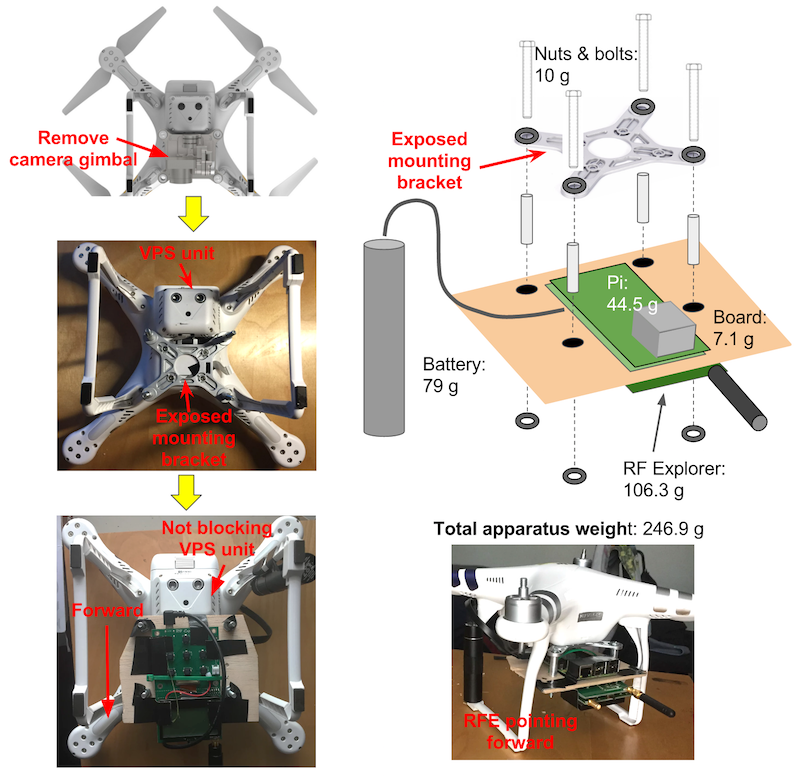
\includegraphics{mounting}}
\end{figure}

 
 A lightweight, balsa wood board was cut to function as the platform for the mounting apparatus. Then, space constraints imposed by the P3A had to be accounted for while considering how to lay out the components of the apparatus. First, in order to attach the board to the bracket, 2 inch bolts with 1 inch spacers were inserted into the openings on the bracket; holes were cut out of the balsa board and the board was fixed in place with washers. This construction was necessitated by the placement of the bracket holes. Laid next to each other, the Pi and the RFE were simply wider than the width of the bracket holes, where bolts would have to secure the board to the drone. Instead, one of the devices would have to go on top of the board and the other on the bottom, which is why the spacers were introduced. Another constraint that presented itself in this revised design was the P3A's VPS sensor attachment, which was fixed to the bottom of the drone towards the rear of the craft and protruded out from the body. Further, if the VPS sensors were covered in any part by the measurement apparatus, optical stabilization would be disabled and the drone might not produce as precise spatial data.  Figure 8b illustrates the mounting apparatus.
 
 The RFE had its antenna fixture at its headDd and its mini USB output at its tail  Because the VPS protruded from the body of the drone and required unobstructed line-of-sight with the ground, the RFE then had to be fixed to the bottom of the board with its antenna oriented towards the front of the craft. The Pi had to be placed on top of the board with its USB ports at the front of the craft, again due to the protrusion of the VPS. A short mini USB cable with right-angle connectors (to minimize sensor obstruction) connected the two components. Additional holes were cut in the board to allow a zip tie to securely tie the components to the board. Lastly, the Anker lipstick battery couldn't fit on the board due to the legs of the craft; instead, it was fixed vertically on the leg of the craft closest to the Pi's power input port. Figure 8a shows the various design constraints imposed by the P3A.
 
 \subsection{Initial Testing and Revised Design}
 The total weight of the measurement apparatus was initially ~380 g, which exceeded the load carrying capacity of the P3A significantly. However, we proceeded to test the flight performance of the mounted P3A to determine the extent to which flight would affected. The drone performed surprisingly well with  this excessive load, with two exceptions. First, since the apparatus was mounted on the underside of the drone, a noticeable "pendulum" effect occurred where the drone swung slightly past it's stopping point at waypoints (see Figure 9). This was more pronounced when flying at heights > 20 ft. As successive tests were performed, the drone began to struggle maintaining its height, likely due to insufficient power from a depleted battery. 
 
 \begin{figure}[h]
 	\caption[Comparison of light paths with heavy and light apparatus]{Flight paths of two test flights with a maximum altitude of 21 ft, one where the measurement apparatus was mounted without modifying the components (yellow) and one after the apparatus was made lighter by 140 g (red). Note the increased stability of the flight path and the more precise turns. }
 	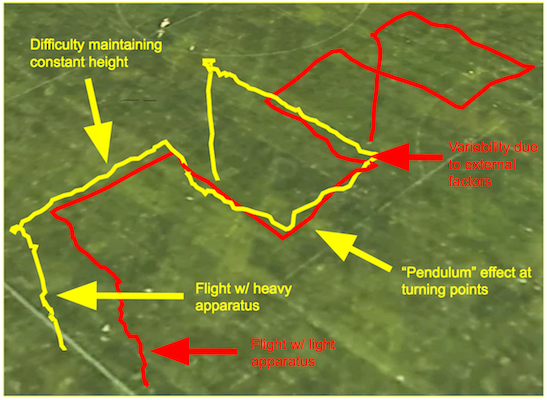
\includegraphics{performance_comparison}
 	\centering
 \end{figure}
 
 A few measures were taken to reduce the weight of the measurement apparatus. The RFE ships with a metal case enclosing its internal circuitry. Additionally, the RFE model used in this project supports measurements in the 900 MHz band as well as the 2.4 GHz band and included specialized antennas for both bands. Both the enclosing case and either antenna (depending on the test being performed) were removed to minimize weight. The final iteration of the measurement apparatus weighed 246.9 grams, well under the 300 g load carrying capacity and about 60 g above the weight of the included camera gimbal. Another adjustment made was increasing the speed of the drone in the Litchi app from 1 mph to 3.5 mph, as extremely slow speeds caused irregular behavior with the drone motors.
 
 \section{Putting it Together: Building the Point Cloud (Proof of Concept)}
Now that the receiver apparatus was mounted on the drone, it was time to see if the DBM system as a whole could generate the desired point cloud of signal propagation. Spatial data would be collected from the drone's flight logs and joined with spectral data gathered from the measurement apparatus. Both systems would have to work in tandem to produce the data we were seeking. 

It was imperative to perform a proof of concept (PoC) test run to validate the functionality of the system and our experimental methodology, and also discover the limitations of the system. To accomplish this, we decided to perform an experiment on an open field without the transmitter component. The transmitter was omitted because we wanted to focus on testing the built components of the project in isolation so it was easier to diagnose issues and observe the limitations of our spectral measurement apparatus. 

\subsection{Setup and Flight Planning}
A set of flight paths using the "lawn mowing" approach (Figure 10) across various heights yielded maximum coverage for consistent data collection and aggregation in 3-D. The mowing approach allows us to systematically sample points in a 2-D plane, as the drone flies in long, parallel strips spaced a few feet apart from one another. Popular drone geographic mapping services such as Skycatch Commander also use this technique to generate a consistent sampling of space. Since our goal is to construct a point cloud in 3-D, we can perform repeated mows at various heights to construct a series of spatial slices which can be stitched together to yield a sampling of 3-D space. Te first step to building the PoC point cloud is to create a 2-D flight path, or slice, as a Waypoint mission in the Litchi app. We can then modify the height of waypoints to gather slices at various elevations.

\begin{figure}[h]
	\caption["Lawn mowing" flight pattern approach]{The "lawn mowing" approach, as viewed from above and from the side. A short lawn mowing flight mission created in Litchi for the proof-of-concept test run.}
	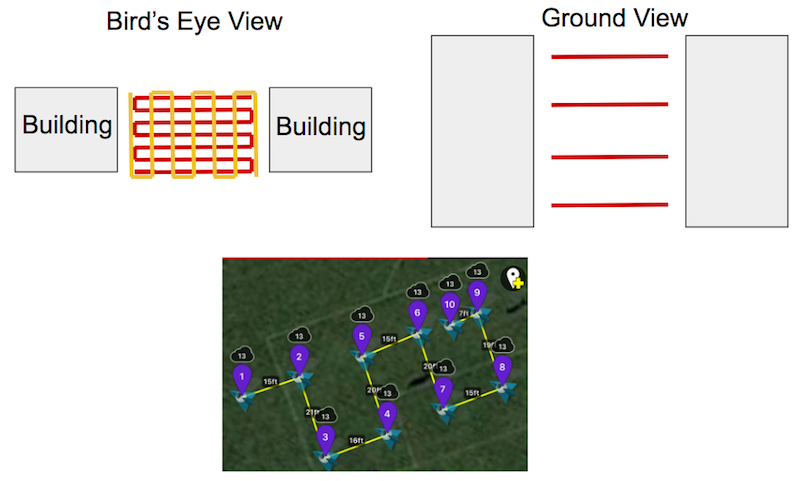
\includegraphics{lawn_mow_PoC}
	\centering
\end{figure}

Due to data on the drone and apparatus being joined on timestamps, the Rapberry Pi's clock had to be aligned to UTC-3 time (see Section 2.6,  "Measurement and Logging Script") and the apparatus had to remain booted from alignment to the end of testing. In order for the Pi to log aligned data throughout the PoC, it had to be synced over a network connection and then left on en route to the testing location, where it would not be possible to connect the Pi to a network. Once the Pi was aligned, it was disconnected from the network and the measurement script was ran. This resulted in lots of extraneous data being logged when the apparatus was in transit; since the Pi had 32 GB of onboard SD card storage, however, storing large amounts of data was not a major issue. 

Upon reaching the testing site, the drone was flown in a lawn mowing pattern at three heights with the RFE measuring in the 2.4 GHz ISM band. The minimum frequency of the RFE was 2406 MHz and the maximum was 2486 MHz. A 2dBi antenna tuned for 2450 MHz was connected to the RFE. Flights would be performed at 6 ft, 11 ft, 17 ft and 23 ft with the drone flying at 3.5 mph. Five flights would be performed autonomously at each height to get a thorough data set over which noise could be smoothed out. Autonomous flights were performed with the drone controller on, in case manual control of the aircraft had to be regained at any point.

In total, 18 flights across the 4 heights were performed. Despite the P3A having state-of-the-art battery life, the drone reached critical battery levels and performed an auto-landing at the configured battery life threshold (see Limitations). The measurement apparatus was left on for the duration of testing, which lasted 2 hours and 1 minute, accounting for transit, setup and flight time. 

\subsection{Processing and Joining Data: Specifics}

Spatial data collected from the drone flights and spectral data logged by the measurement apparatus had to be extracted, aligned and joined with each other to output the point cloud. Flight logs, each corresponding to a single flight, were downloaded from the Airdata UAV repository while spectral data was collected in a single large file on the Raspberry Pi. The Pandas data analysis framework was used to read the data sets from files into an iPython notebook and perform operations on the data; visualization was done with a combination of matplotlib and plotly.

Since data sets have to be joined on equal column values, the timestamps in spatial and spectral had to be aligned to a common format; for this project, timestamp columns were aligned to the nearest 100 ms and joined using an inner join. The drone flight logs saved rows of data with a 10 Hz update rate. Time information was split across two columns, with a "flight\_time" column specifying how long (in milliseconds) the flight corresponding to the log file had been in progress and a "datetime(utc)" column logging the UTC time with second precision. Since flights were performed autonomously, rows in the flight log corresponding to auto take-off and landing flight states were filtered out. The resulting data set captured the entirety of the drone's waypoint mission flight. Flight time values were rounded to the nearest 100 ms and concatenated with values from the datetime column to form a consolidated timestamp field that could be joined on. Similarly, the RFE had an update rate of 5 Hz and each row in the measurement log file was timestamped with microsecond precision. These timestamps were also rounded to the nearest 100 ms. 
The spectral data was filtered to only include rows collected when the drone was flying.

\begin{figure}[!ht]
	\caption[Data processing pipeline]{The complete data processing pipeline required for this project. Left: Spatial data processing on flight logs gathered from Airdata UAV and the Litchi app. Data from each flight is passed through this pipeline and appended to generate one table with all flight data. Right: Spectral data pipeline from the measurement apparatus. Inner join results in one table combining spatial and spectral data.}
	\centerline{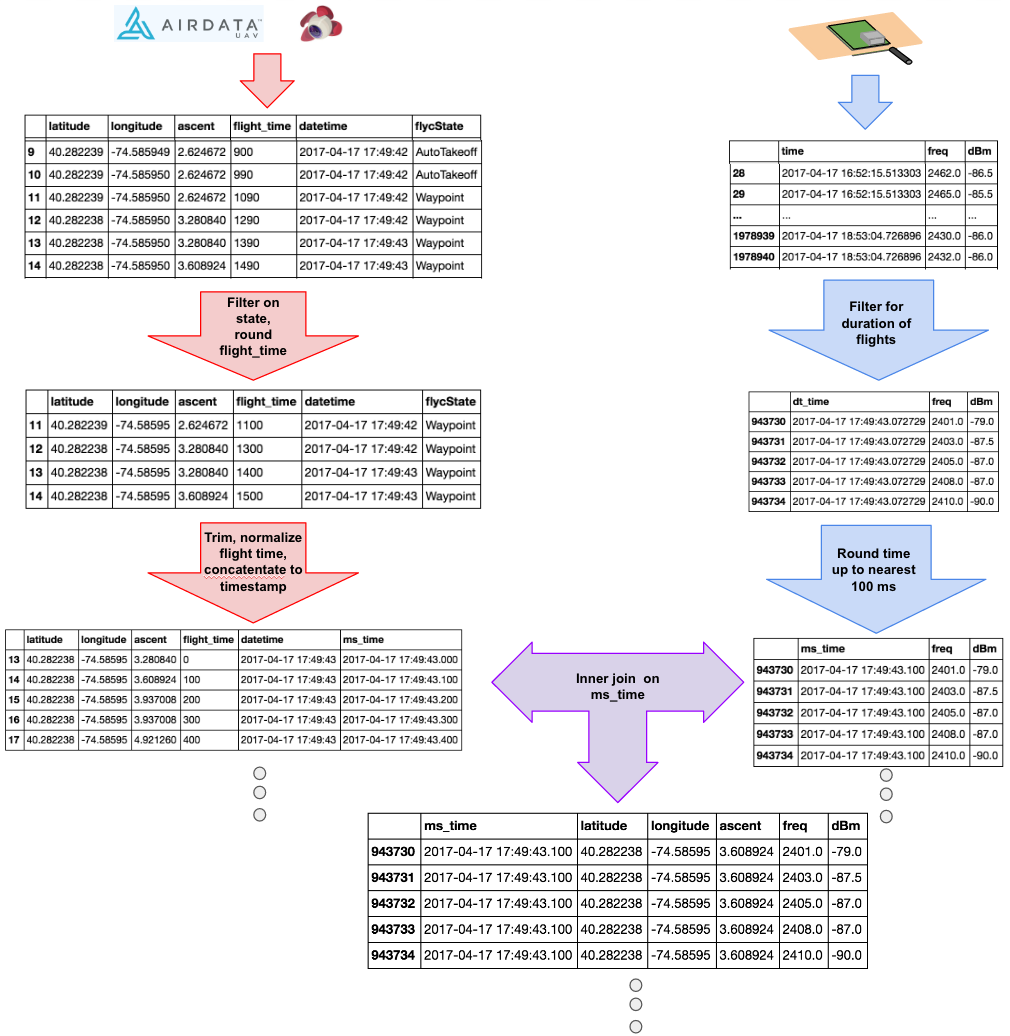
\includegraphics{data_pipeline}}
\end{figure}
\pagebreak

Once timestamps were aligned across the datasets, an inner join was performed to join the data sets. An inner join was preferred so that empty rows resulting from an outer join with only spatial or spectral data could be avoided in practice. Aligning the timestamps with each other resulted in > 99\% of spectral data rows being included in the final joined data set. The size and update rate of the resulting dataset was limited by the slower update rate (~5 Hz) of the RFE. Since the P3A was flown at a speed of 3.5 mph, an update rate of 5 Hz translates to consecutive data points being spaced about 1 ft apart. Figure 11 describes the full data pipeline in more detail.

\subsection{Visualizing the Point Cloud}
Once the spectral and spatial data were joined, a few small tweaks and additions were needed to add context to the dataset before it could be visualized as a point cloud. The latitude and longitude columns of the dataset were normalized to feet for consistency with the height data with the minimum values corresponding to 0 ft. Further, before plotting, an additional row with populated spatial fields and null spectral fields was added to indicate the position of the drone controller (and operator) relative to the measured space. 

With these modifications, the joined data was ready for visualization and analysis. A 3-D scatter plot (Figure 12) was constructed using Plotly, where points were colored relative to the maximum and minimum signal strength values measured during the test flights. 

\begin{figure}[!h]
 	\caption[Point cloud visualization from proof-of-concept 2.4 GHz test]{Visualizing a point cloud of signal strength measurements from the 18 flights performed for the Proof-of-Concept test run. Note the flight pattern in the "Bird's Eye View", which is the real world  resulting from the Waypoint mission in Fig 10. Flights were performed at heights of 8 ft, 13 ft, 20 ft, 26 ft.}
 	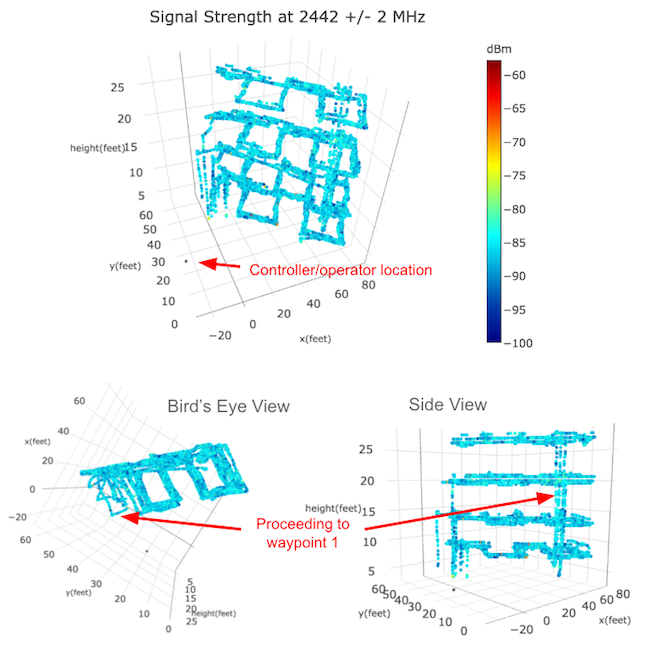
\includegraphics{PoC_1}
 	\centering
\end{figure}

\subsection{Analyzing the PoC Propagation Data}
Data collected during the PoC was gathered in the absence of a dedicated transmitter, so the point cloud measurements were representative of two sources of noise: ambient noise from the environment and transmissions from the drone controller. While the PoC was successful in terms of validating the functionality of the implementation and data processing pipeline, it also revealed large sources of noise which necessitated hardware changes moving forward.

As mentioned earlier, the 2.4 GHz ISM band is overcrowded due to the many ubiquitous consumer electronic devices operating in it. Because of this, there was a consistent ambient noise level across the 2.4 GHz spectrum. The RFE is sensitive to signals as weak as -120 dBm, but signal readings of -80 dBm were extremely common across the 2.4 GHz band. For example, the mean signal strength detected at 2442 +/- 2 MHz was -87 dBm, with a $\sigma$ of just 2.9 dBm. In the point cloud (Figure 13), we can visualize this ambient noise as a steady sea of interference present across all spatial measurements.

\begin{figure}
	\caption[Closer analysis of PoC point cloud at different frequencies; identifying noise]{Top: Point cloud representations of measurements at 2412, 2442, and 2472 MHz. Note that 2472 MHz is within the Lightbridge channel setting of the P3A controller. Evidence of high measurements due to the FHSS control signal are highlighted at lower frequencies. Bottom: Signal strength distributions at the various frequencies. Note the persistent ambient noise profiles across the 2.4 GHz band. }
	\centerline{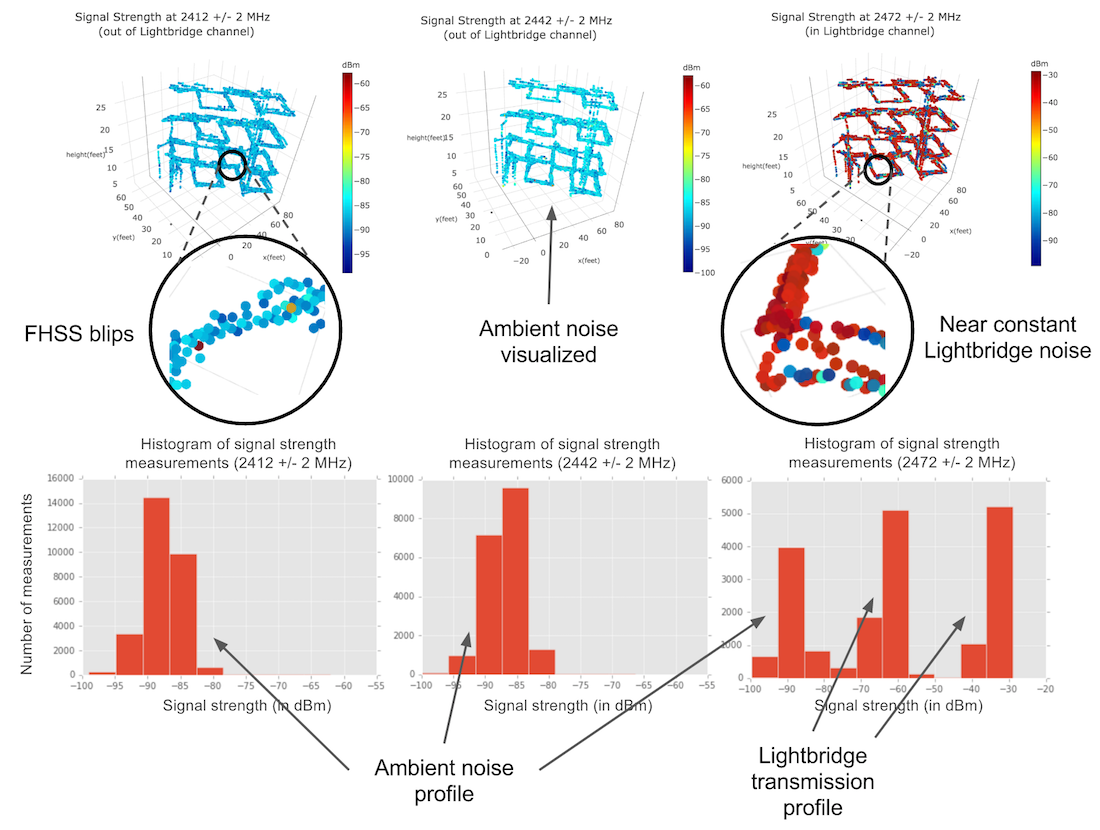
\includegraphics{PoC_2}}
\end{figure}

Beyond a base noise environmental noise level, the P3A and its controller transmit their own wireless signals for control and data transmission. Since the P3A is designed with photography in mind, it uses LightBridge, DJI's proprietary data transmission protocol, to beam a live video feed from the camera to the controller. LightBridge operates in the 2.4 GHz ISM band and the P3A begins transmitting data when it establishes a preliminary connection with the controller. The frequency channel over which Lightbridge is operating can be coarsely configured; for all the experiments, Lightbridge channel 20 (2471MHz - 2482MHz)\cite{p3a} was selected. The aircraft and the controller transmit over this channel continuously; this is evident in the constantly high (> -40 dBi) point cloud measurements for frequencies falling withing the range of Lightbridge channel 20 (see histogram \#3 in Figure 13). Despite the built-in camera being disconnected and no video being available, the P3A continues to transmit data from the craft's telemetery and navigation systems in the configured Lightbridge channel. While the data transmission frequency range can be manually set, the P3A receives remote control signals from the controller at non-configurable, variable frequencies throughout the 2.4 GHz ISM band. A frequency hopping, spread spectrum (FHSS) method is used for control transmissions, where data is sent over rapidly changing frequencies between the craft and the controller, randomly hopping across the 2.4 GHz ISM band. While these transmissions are drowned out by constantly strong signals in the data broadcasting frequencies, they are briefly observable in the mid-to-lower reaches of the RFE's measured spectrum (see point cloud \# 1 in Figure 13). For example, at 2412 +/- 2 MHz, the mean signal strength measurement was -87.6 dBm with a $\sigma =$2.9 MHz; however, there were 58 measurements out of 28695 that registered greater than -70 dBm. The presence of these two different sources of noises meant that data collection would be noisy regardless of where in the 2.4 GHz band we measured.

Ambient noise in the 2.4 GHz band was expected, but the prevalence of controller transmissions across the measured band necessitated changing frequency bands moving forward. Since the P3A controller was the source of noise, experiments were performed with the controller off but these presented other unexpected implementation challenges. The drone transmitted navigational data to the Litchi app via the controller; flying waypoint missions with the controller off resulted in empty flight logs. Unfortunately, the built-in logs produced by the P3A are saved as .DAT files which require third-party scripts to decode; the programs built by the Phantom pilot community all lacked data elements needed to generate the point clouds. 

To get around these issues in the 2.4 GHz band, the 900 MHz ISM band was used moving forward. The 900 MHz (902 MHz - 928 MHz) band is much narrower than the 2.4 GHz band (2400 MHz - 2500 MHz) and used far less in the consumer electronics space. Further, a signal in the 900 MHz travels farther and features better penetration characteristics than a signal in the higher frequency ISM bands. Reduced noise and increased penetration are preferred characteristics for mesh network links; as a result, companies like Ubiquiti offer many wireless networking devices operating in the 900 MHz spectrum. Further, the RFE featured dual-band measurement capabilities allowing us to measure in this band without any other implementation modifications.

\section{Introducing a Transmitter: Measuring Real-World Propagation}
With the proof-of-concept completed, a dedicated transmitter could be added to the experimental methodology, allowing us to collect real-world, 3-D propagation data. The Ubiquiti NanoBridge M900 transmitter was situated in an open field; point clouds of signal strength measurements were collected with the transmitter sending data and compared with measurements gathered while the M900 was switched off. The goal of this real-world field test was to observe whether transmitter propagation characteristics would present themselves in the data and identify necessary changes to transmitter configuration and experimental methodology before testing in an urban setting.

\subsection{Configuration and Experimental Methodology}
To observe the propagation pattern of the M900, the transmitter would have to be configured to transmit data continuously and measurements collected in the presence and absence of transmission. Ubiquiti's airOS firmware was used to log onto the transmitter and change settings. First, the M900 was set to Access Point (AP) mode; when configured as an AP, the link intermittently broadcasts packets containing identifying information (such as its network name) so that devices in the surrounding area can establish a connection. Then, the transmitting frequency, channel width, and output power of the AP can also be set. The center frequency of the device was set to 914 MHz and the channel width set to 5 MHz; the default output power of 28 dBm was selected. Since the 900 MHz ISM band is very narrow, these settings allowed us to sample across the entirety of the band and capture measurements at frequencies less than, within, and greater than the transmitting channel. To simulate continuous data transmission, a  non-terminating \texttt{ping} process was ran on the M900 by SSH-ing onto the device. Specifically, \texttt{ping -s 65007 192.168.1.21} was issued so that large ICMP packets would be broadcasted out of the M900's wireless interface. 

Lawn mowing flight patterns were interlaced (as in the Bird's Eye View in Fig 10), forming lattice-like 2-D coverage at various heights. In order to capture any noticeable difference in signal propagation on an open field, a relatively large spatial area (compared to the PoC test) had to be sampled at a distance from the transmitter. A simple war walking exercise was performed while the M900 was on to determine rough boundaries where differences (> ~20 dBm) in max signal strength measurements could be observed. 

Once these flight and device parameters were established, on/off experiments were performed at heights of 9ft, 16ft, and 23 ft. Two flights, providing lattice-like coverage, were performed at each height with the transmitter on and another two flights were performed at each height with the transmitter off. 

\subsection{Visualizing and Analyzing Open-Field Propagation}
Ideally, the open-field test measurements would reveal a propagation picture in 3-D space consistent with the radiation patterns of the M900 (shown in Fig 4). Due to low noise in the 900 MHz band, low signal strengths close to the sensitivity limit (-120 dBm)  of the RFE were expected in flights conducted while the M900 is turned off. 

Point cloud measurements were visualized separately in sets where the transmitter was on versus when the transmitter was off (see Figure 14). Initially, measured values at the center frequency were plotted in the presence and the absence of the transmitter. When the M900 was off, the data aligned with our expectations; the mean value registered by the RFE at the center frequency (914 MHz) was -114.6 dBm with a $\sigma$ of 1.88 dBm. In cases where the transmitter was on, naively considering measurements at the center frequency (Figure 14) was not an effective approach. While the data collected during transmission contained many high signal strength measurements indicating that the M900 signal was propagating through the space, a clear propagation pattern could not be determined due to a large fraction of low (< -110 dBm) measurements. For example, 9.48\% of measured values at 914 MHz were > -90 dBm but over 50\% of values were also < -114 dBm (see histogram \#1 in Figure 14).

\begin{figure}
	\caption[Point cloud visualization of 900 MHz open field test]{Top left: Measured signal strength values at 914 MHz when the M900 transmitter was on and placed approximately 15 yards from the near-edge of the lattice. (Inset: an example of high and low measured values occurring periodically in the point cloud) Top right: Measured values at 914 MHz when the transmitter was off. Bottom left: Distribution of signal strength values in the point cloud above. Note the large number of extremely low measured values }
	\centerline{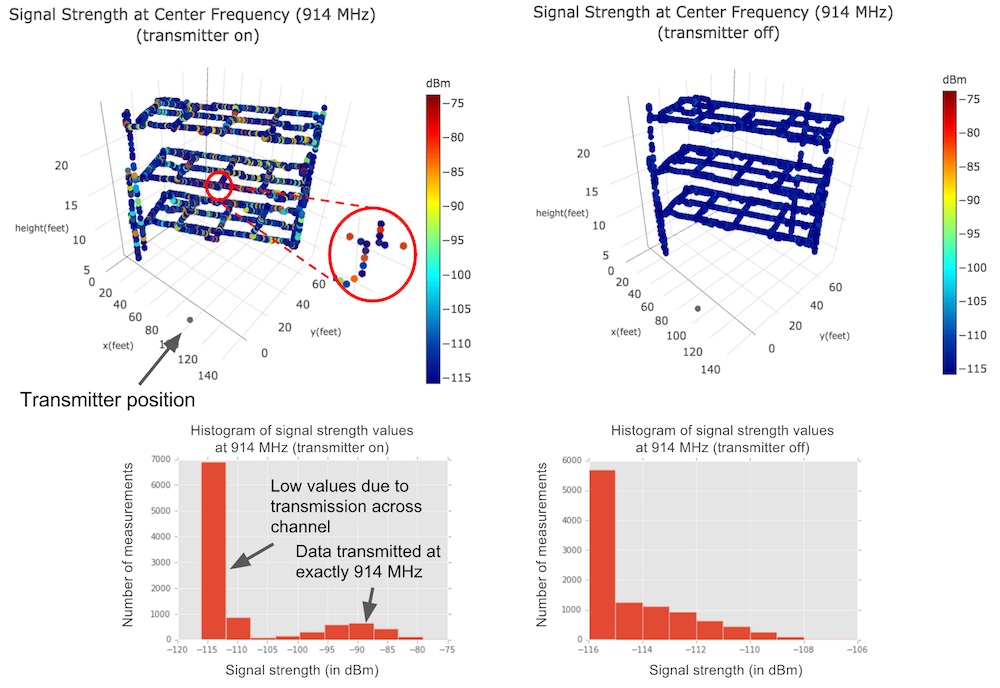
\includegraphics{Sexton_1}}
\end{figure}

A high density of low signal strength values would make it difficult to characterize propagation in an open field, much less an urban environment. This behavior was a result of the M900 being designed as a wireless link and not a signal generator. The M900 constantly transmitted in its configured channel but not necessarily at the exact same frequencies each time. In fact, war walking and monitoring using the RFE's on-screen display revealed that a strong signal (> -70 dBm) was being transmitted at some frequency in the range $[center\_freq - 1 \text{MHz}, center\_freq + 1 MHz]$; this was either the result of the M900's hardware design or the sampling rate of the RFE (or both). 

To account for this transmission behavior, maximum signal strength measurements within the transmitting channel were plotted (see Figure 15), as opposed to all measurements at the center frequency. The point cloud data set was filtered for all measurements at frequencies within the 914 MHz $\pm$ 2.5 MHz range, to match the M900 configuration.  A \texttt{GROUP BY} operation was performed on the point cloud data set, grouping measurements with the equal timestamps; the maximum signal strength measurement in each group was selected to populate the final data set. 

\begin{figure}
	\caption[Point cloud visualization of max values from 900 MHz open field test]{Top: Point cloud generated by plotting maximum signal strength values in the transmitting channel. Bottom left: Propagation pattern of the M900 in the azimuth and (Bottom center) elevation planes. Note the directional nature of radiation, and the side lobes, which can be found on the plot relative to transmitter orientation. Bottom right: Distribution of plotted values. Note the lack of noise relative to distributions in Fig 14.  }
	\centerline{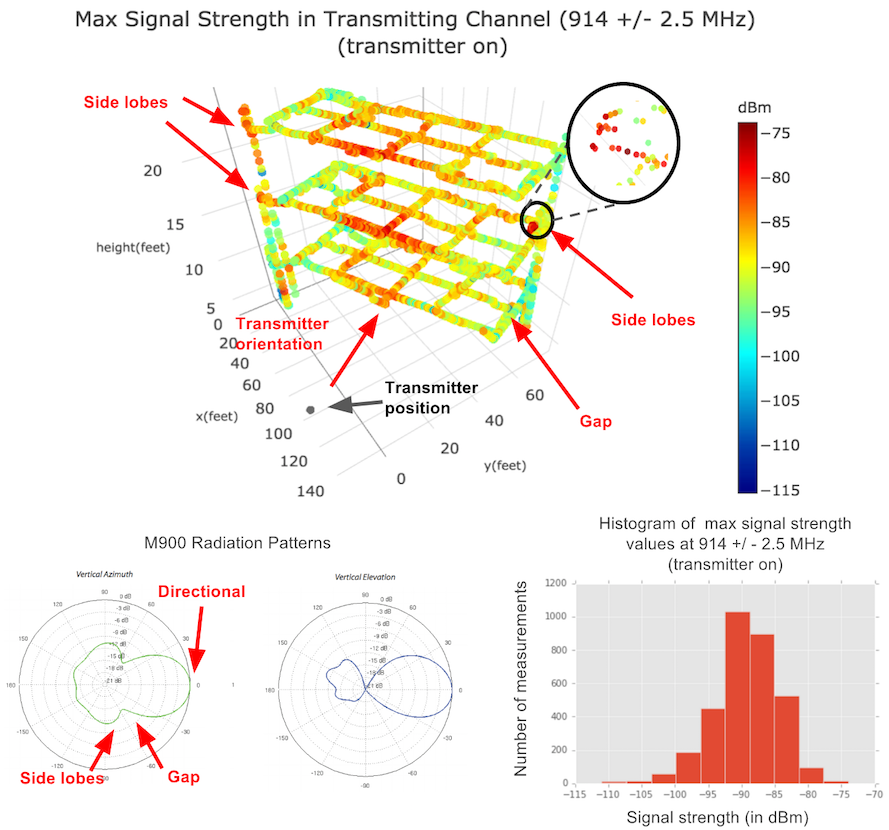
\includegraphics{Sexton_2}}
\end{figure}


Plotting the maximum signal strength within the transmitting channel at each spatial point yielded a very robust data set where propagation characteristics could be visually identified (see annotations in Figure 15). The distribution of signal strength values resembled a bell curve (Figure 15) with a mean strength of -89.4 dBm and $\sigma$ = 4.9 dBm. With this point cloud, we could observe the radiation pattern (Fig 15) of the M900 in the azimuth plane measured in 3-D space. The primary directional lobe centered at 0 degrees could be observed in the highest measured values being directly in front of the transmitter. Interestingly, the M900 features secondary lobes at 90 degrees and -90 degrees. Relative to the orientation of the transmitter, these lobes presented themselves as small clusters of high (> -80 dBm) signal strengths at the widest reaches of the measured spaces. In between these areas and the center of the point cloud, was a span of lower measured values; this can be attributed to the low-output power gap at approximately 60 degrees and -60 degrees relative to transmitter orientation. Using this analysis method allowed us to observe real world propagation behavior in a low-noise environment and would serve as the basis for further experimentation and analysis in an urban setting.

\section{Measuring Propagation in Urban Environments: Friend Center}
Observing expected transmitter behavior in a controlled field setting gave us the confidence to proceed with measuring in an urban setting on campus. The goal of performing an experiment in the presence of features is to assess how certain urban structures affect real-world propagation. This can be analyzed by measuring signal strength in the presence of an active transmitter placed at a given location and orientation and comparing measurements taken in an open field with the same spatial relationship with the transmitter. Once this data was collected, it could be aggregated and normalized to inform how much a certain transmitter and urban configuration worsens propagation relative to ideal conditions; multiple configurations can be tested and the most favorable selected as the layout of a mesh network in the space.

\subsection{Configuration and Experimental Methodology}
Location was an important consideration for this phase of testing, as we wanted to simulate a real-world use case of wireless links in an urban setting, as well as observe the effects of different features on 3-D signal propagation. As part of a mesh network, a wireless link would likely be placed outdoors on the side or roof of a structure , or indoors near a window. If the link was configured as an access point (AP), it would be able to connect to other APs and form hops in the mesh network, or connect directly to links configured as stations; these stations could then be connected to a wireless router to provide Internet to end users. Other links in the surrounding urban area could be placed in an unorganized manner by users, often at varying heights and orientations.

The open courtyard feature created by the Friend Center, Computer Science building, and Sherrerd Hall featured several interesting urban characteristics and could be used as a model simulating a real mesh network use case. First, the buildings are situated in fairly close proximity to each other and are all three or four stories in height; this limited the scope of our experiment and made it viable to construct a 3-D point cloud mapping the entire area. Further, certain sections of the space don't have direct line-of-sight (LOS) with other sections; placing a transmitter strategically in these locations could provide insight on how obstacles affect propagation throughout the space. 

One of the limitations of data collected in the open field test was the sparsity of the spatial data; for this simulation, we flew the drone in a more dense flight pattern. In the field test, parallel sweeps in the lawn mowing pattern were drawn 14-23 ft apart; at Friend Center, parallel lines were spaced only 7-10 ft apart. The overall 2-D area sampled was also larger than in the field test because we wanted to gather measurements throughout the entire space between the three buildings. Since the drone can't automatically detect and avoid obstacles, the space was split into three sections (which will be referred to as section 1, 2, and 3, denoted in Figure 16) separated by various features. Two rows of trees and the three buildings served as features that we could fly in front of and behind to get a robust understanding of propagation in this location.

\begin{figure}
	\caption[Friend Center planning and flight path.]{The Friend Center courtyard urban feature; the pink areas were sampled. The transmitter was placed in one corner of the courtyard approximately 70 ft from the rightmost spatial section.}
	\centerline{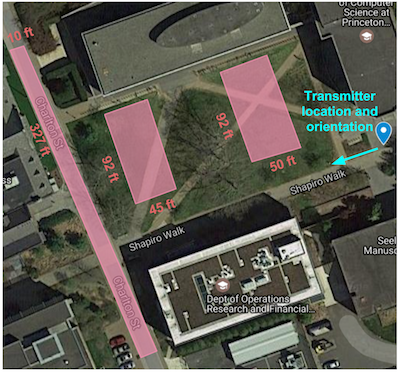
\includegraphics{friend_1}}
\end{figure}

Flights in the Friend Center courtyard were performed with the M900 always on with the same configuration as the open field test. The transmitter was always on in this round of testing because the field test revealed that  ambient noise in the 900 MHz is generally non-existent; before flying near Friend Center, a manual war walking test with the RFE confirmed that there was no noise in the sampled spectrum in this location either. Testing needed to be limited due to battery life. With a denser flight path over a larger spatial area, sampling the entire space twice with the transmitter on and off was not feasible due to increased flight time.

\subsection{Visualizing and Analyzing 3-D Propagation in an Urban Space}
Flight were conducted at heights of 9 ft, 16 ft, and 23 ft above the three sections of the Friend Center courtyard. The transmitter was placed next to the Computer Science building facing into the courtyard and continuously broadcasted \texttt{ICMP} packets with a center frequency of 914 MHz and a channel width of 5 MHz; it was approximately 70 ft away from the first spatial section. Several days after flying at Friend Center, another identical test was performed in an open field, which served as a control experiment. The same transmitter settings were used in this control field test, and the relative positioning of the transmitter and the spatial sections was the same. 

We expected the measured signal strength values to be higher in the control field test and lower in the urban setting. The trees and structures in the space could absorb\cite{reflections} the 900 MHz signal and prove to be unfavorable characteristics for propagation. The technique of filtering the maximum measured signal strength within the transmitting frequency that yielded more robust results in the open field test was also used with the data gathered in this set of experiments. 

The data painted a completely different picture than what we expected, however; we aggregated the measurements taken in each section of the urban experiment and compared their averages with the corresponding sections of the control test. Upon visual inspection, measured values were greater throughout the urban space than in the open field. The data collected in the Friend Center courtyard (Figures 17 and 18) aligns with what we expected going into the simulation. We expected the strongest signal strength measurements to be nearest to the transmitter in section 1; there were no obstacles between the M900 and section 1. Section 2 was almost uniform, with a mean signal strength of -95.5 dBm and a $\sigma$ of 4.7 dBm. Section 3 was particularly interesting. The middle of section 3 looks like an extension of section 2, but the far reaches of the flight path indicate reduced propagation due to Friend and Sherrerd Hall (see Figure 18).
 
\begin{figure}
	\caption[Bird's eye view and distributions of Friend Center and field control test point clouds.]{Top left: Birds-eye view of the propagation point cloud for the urban simulation conducted in the Friend Center courtyard. Note the low measured values in the measurement slice behind Sherrerd and Friend halls. This is likely due to LOS obstruction by the structures.Top right: Histogram of measured values in the Friend Center courtyard across all sections. Bottom: Birds-eye view of the propagation point cloud for the control experiment performed on an open field. Note the lower values throughout the point cloud compared to the data at Friend Center. Bottom right: Histogram of measured values in the control field test across all sections. }
	\centerline{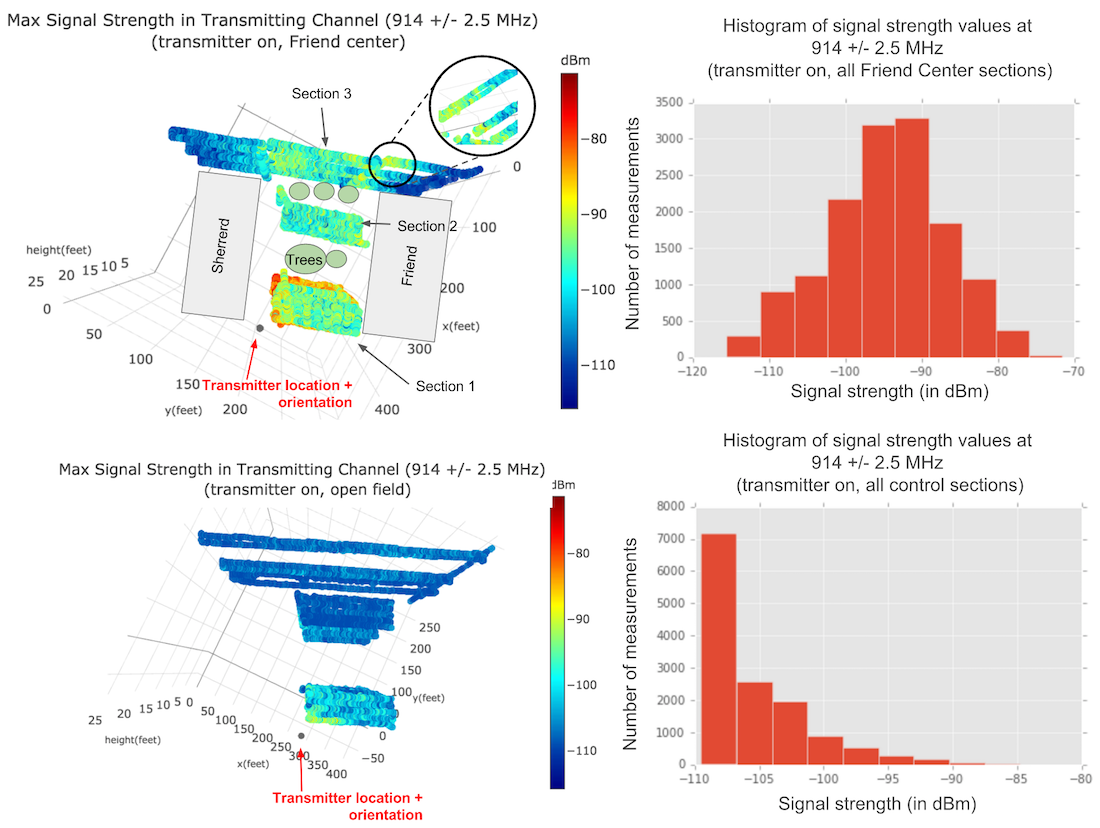
\includegraphics{friend_2}}
\end{figure}

\begin{figure}
	\caption[Side view of Friend Center and field control test point clouds.]{Left: Side view of the propagation point cloud for the urban simulation in the Friend Center courtyard. Note the very high values closest to the transmitter. Right: Side view of the propagation point cloud for the control experiment in an open field. The highest relative values are closest to the transmitter but they are lower than the corresponding measurements in the urban space. }
	\centerline{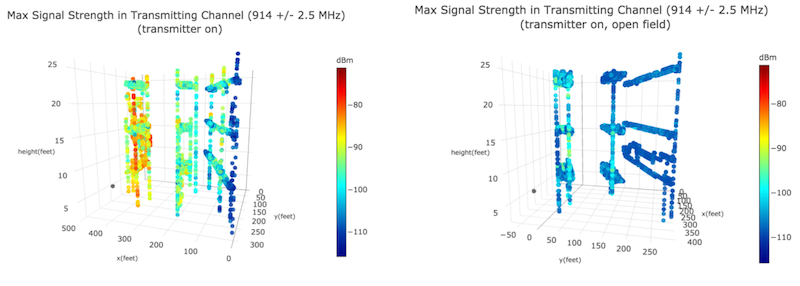
\includegraphics{friend_4}}
\end{figure}

\begin{figure}
	\caption[Distributions of the measurements gathered at sections 1-3 at Friend Center and in the field control test]{Distributions of the measurements gathered at sections 1-3 at Friend Center (left) and in the field control test (right), demonstrating one way to spatially aggregate point cloud measurements. These distributions can be used to analyze the amplifying effect of the Friend Center courtyard. }
	\centerline{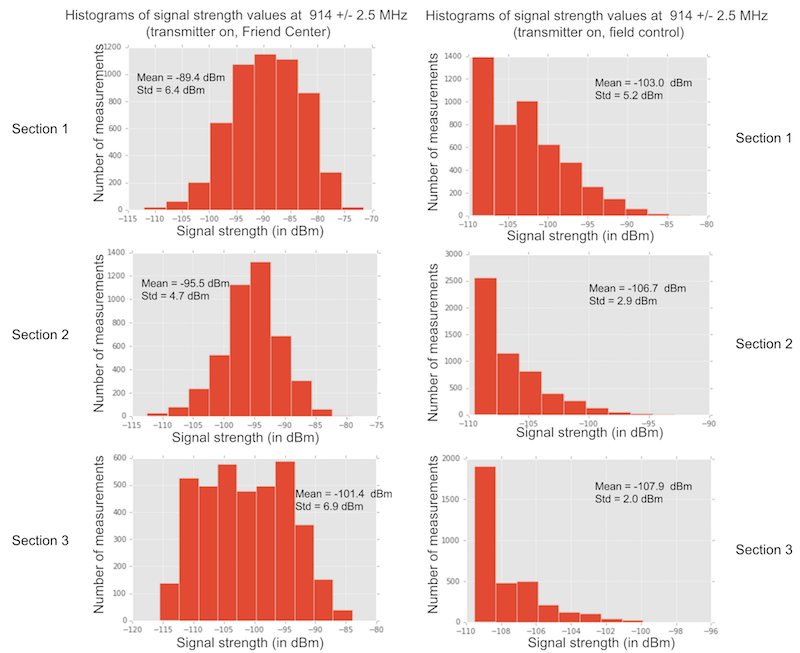
\includegraphics{friend_5}}
\end{figure}

While these insights aligned with our expectations, we did not expect measured values in the Friend Center courtyard to be greater than those in the open field test. Section 1 in the courtyard had a mean signal strength of -89.4 dBm, while Section 1 in the control test had a mean signal strength of -103.0 dBm (see Fig 19). The mean measurements were lower in the other two sections as well. This discrepancy could have resulted from a few different factors. First, Sherrerd Hall, Friend Center, and the CS building may have provided reflective surfaces for the 900 MHz to get directed back into the center of the courtyard. Friend Center and Sherrerd Hall both have glass and metal exteriors, which may contribute to signal reflection\cite{reflections}. Further, the CS building was to the right of the transmitter in the simulation; it may have reflected some of the radiation from the M900's side lobes into the middle of the courtyard. These reflected waves could have positively interfered with the directional transmission of the M900 and produced higher average measurements per section. Lastly, a new RF Explorer (but the same model) was ordered between the urban testing and the control testing. This may have contributed to some variation across the two plots, but it is unlikely to be the sole cause for the difference.This is because we can compare the mean value of section 1 in the control test with the open field testing (see Figure 15). The sweep furthest from the transmitter in the open field testing was about the same distance as section 1 in the control testing was to the transmitter; the measured values across the two tests are comparable at similar distances from the transmitter.

By aggregating per spatial section, we were able to directly compare the control experiment data with the measurements gathered in an urban setting. Aggregating over the three spatial sections allowed us to normalize the data and directly determine the effects of the urban layout on propagation. In terms of raw signal strength, the urban features actually amplified the 914 MHz in each section relative to the same spatial and spectrum configuration in an open field.
	
\section{Conclusion}
Our goals for this project were to build a drone-based measurement (DBM) system capable of robustly measuring radio propagation in an urban space to better inform wireless mesh network design. We were able to successfully implement the DBM system to generate a 3-D point cloud of signal strength measurements in an urban space. A measurement apparatus consisting of a spectrum analyzer and a Raspberry Pi was mounted to a drone which flies in a strategic path to sample a 3-D space. Many implementation challenges presented themselves, including actually mounting the apparatus, joining spatial and spectral data, and devising the experimental methodology to gather the data. 

Several experiments were performed with the completed DBM system. First, a proof-of-concept sampling of ambient noise and drone controller transmission was performed on an open field in the 2.4 GHz ISM band. This noise, particularly drone transmission, was profiled and found to be prohibitively high to continue measurements in the 2.4 GHz band. After switching transmitter and receiver equipment to devices operating in the 900 MHz band, an open field test measuring propagation from a transmitter was performed. The Ubiquiti M900 was used and the resulting point cloud was able to detect characteristics of the M900's propagation pattern in the sampled 3-D space. This validated our approach and allowed us to identify an urban feature on Princeton's campus and simulate signal propagation from a wireless link; we used the DBM system to perform a robust measurement campaign of this simulated use case.

We were able to conduct a thorough measurement campaign in the Friend Center courtyard, partially enclosed by Sherrerd Hall and the Computer Science building. Testing was split into three sections based on the obstacles in the space and a control measurement campaign was replicated on an open field. The distribution of signal strength measurements in each section of the Friend Center courtyard was compared with the distribution in the corresponding section of the control field test; interestingly,  measured signal strength was greater across all sections in the urban space, which was unexpected. 

Aggregating the point cloud data per section measured served as a valuable way to compare data gathered in the urban simulation at Friend Center with the open field control test. Splitting the sampled space into equal volumetric sections with the same relative positions and transmitter configurations could be a useful way to compare the effect different transmitter locations and settings of propagation in the same urban space.

In combination, this system enables wireless mesh network designers to gather a complete data set informing the placement of wireless links in an urban network. Our hope is that such a system can be used to gather vast amounts of data in the future, where effects on propagation can be characterized by urban feature and transmitter configuration. Companies hoping to build wireless mesh networks to disrupt the oligopoly of last-mile Internet delivery can draw from this data to design more robust and performant mesh networks.

\section{Limitations}
The drone-based measurement system certainly had limitations, especially in battery life and the resulting sparsity of data in the propagation point clouds. In order to get a dense point cloud with consecutive data points close together (< 1 ft apart), the drone has to be flown at speeds less than 4 mph. Sampling a large spatial area like the Friend Center courtyard at varying heights with a slow flying speed resulted in demanding flight times. Extra batteries were purchased but even added capacity was hardly enough to complete one full sampling of the Friend Center courtyard with a denser flight pattern. Further, the amount of time available to test due to drone flight restrictions imposed by the University prohibited us from recharging batteries for prolonged testing.

\section{Future Work}
In addition, to generating more dense point clouds, a variety of data analysis techniques could be applied to the datasets to yield more insight. For example, a more dense data set would enable us to split the 3-D space into small cubes (e.g. 1000 cubic feet)instead of large spatial sections. Then, cubes could be classified; for example, cubes could be tagged as "window" cubes, if they're near windows of buildings in the urban space. Since mesh network users would likely have wireless links in their windows, signal strength values in these cubes could be weighted more heavily than other cubes in the space when comparing transmitter configurations.

\begin{figure}[]
\caption[Future work includes comparison with ray tracing models]{Example output of ray tracing models\cite{raytrace}. Real-world 3-D measurements by systems such as the one we built could then be compared to predicted outcomes.}
\centerline{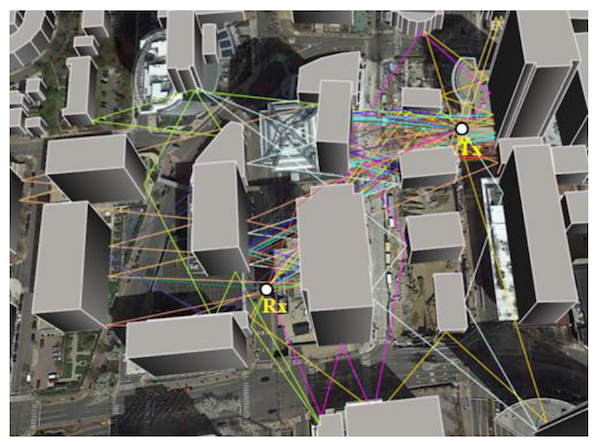
\includegraphics{ray_tracing}}
\end{figure}

More work could also be done in comparing measured propagation with expected propagation from ray tracing models. Yun and Iskander have created sophisticated ray tracing\cite{raytrace} simulations in urban settings using spatial data available in Google Earth (displayed in Figure 20). Future versions of this work could compare the signal strength predicted by ray tracing and other propagation models with the real-world measured signal strength; this can inform how accurate these propagation models are as well. Over time, with enough data collection and comparison with existing models, urban features (courtyards, slits between buildings) could be characterized with their precise effects on propagation given different transmitter locations. Then, programs could be developed to dynamically and accurately display the 3-D propagation of a wireless link transmission through an urban space; companies could use this trove of characterized data to quickly expand and build large, robust wireless mesh networks.

\bstctlcite{bstctl:etal, bstctl:nodash, bstctl:simpurl}
\bibliographystyle{IEEEtranS}
\bibliography{references}

\end{document} 

